\documentclass{article}
\renewcommand{\contentsname}{Contenuti}
\usepackage[utf8]{inputenc}
\usepackage{graphicx}
\usepackage{float}
\usepackage[export]{adjustbox}
\usepackage[font=small,labelfont=bf]{caption}



\title{Progetto in Java per la gestione di un'auto a guida autonoma}
\author{Elisa De Filomeno}
\date{A.A. 2020-2021}

\begin{document}
\maketitle
\newpage
\tableofcontents
\newpage 


\section{Introduzione}
L'elaborato consiste nella realizzazione di un progetto di microprogettazione scritto nel linguaggio Java. Esso simula, in modo semplificato, il meccanismo di funzionamento della guida autonoma di un veicolo. L'obiettivo è quello di fornire una struttura adeguata per problemi di gestione analoghi, mostrando il modo con cui le varie classi si relazionano tra loro attraverso la combinazione dei design pattern Iterator, Observer e Builder.  
Seguendo l'impianto fornito si favorisce una possibile realizzazione di implementazioni più complesse delle singole funzioni o l'aggiunta di ulteriori classi.

\section{Design Patterns}


\subsection{Observer}
Si tratta di un pattern comportamentale che viene utilizzato quando si vuole realizzare una dipendenza uno-a-molti, in cui il cambiamento di stato di un soggetto (Subject) viene notificato a tutti oggetti (Observer) interessati.
\subsubsection{Struttura}
\begin{figure} [H]
\begin{center}
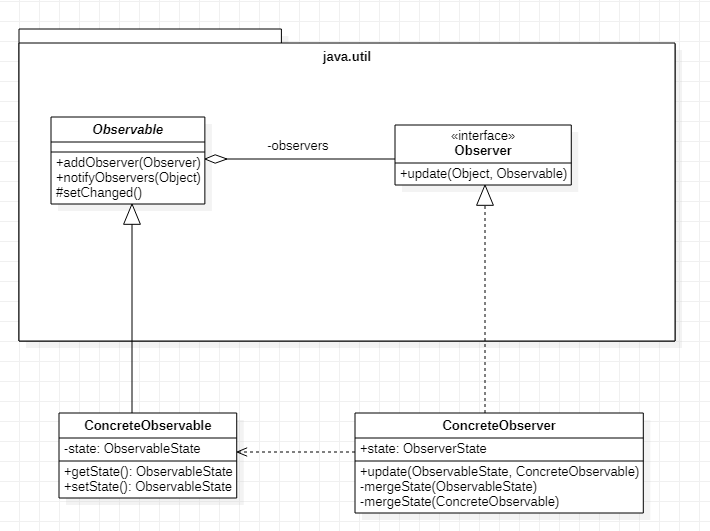
\includegraphics[scale=0.5]{ObserverClassDiagram.png}
\end{center}
\caption{Observer Class Diagram}
\end{figure}
\begin{figure} [H]
\begin{center}
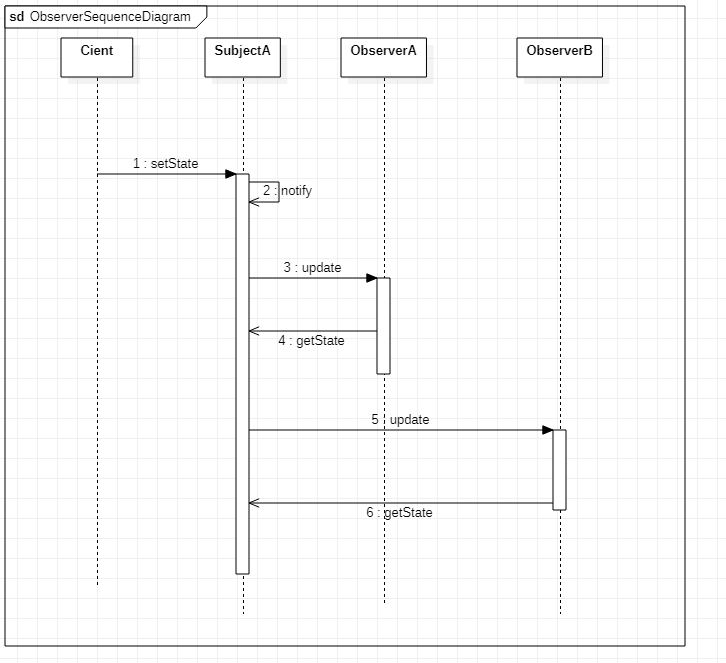
\includegraphics[scale=0.5]{ObserverSequenceDiagram.png}
\end{center}
\caption{Observer pull mode Sequence Diagram}
\end{figure}

\subsubsection{Partecipanti}
Questo pattern è composto dai seguenti partecipanti:
\begin{itemize}
  \item Subject: espone l’interfaccia che consente agli osservatori di iscriversi e cancellarsi; mantiene una reference a tutti gli osservatori iscritti
  \item Observer: espone l’interfaccia che consente di aggiornare gli osservatori in caso di cambio di stato del soggetto osservato.
  \item ConcreteSubject: mantiene lo stato del soggetto osservato e notifica gli osservatori in caso di un cambio di stato.
  \item ConcreteObserver: implementa l’interfaccia dell’Observer definendo il comportamento in caso di cambio di stato del soggetto osservato
\end{itemize}
\subsubsection{Conseguenze}
Tale pattern presenta i seguenti vantaggi/svantaggi:
\begin{itemize}
  \item Astratto accoppiamento tra Subject e Observer: il Subject sa che una lista di Observer sono interessati al suo stato ma non conosce le classi concrete degli Observer, pertanto non vi è un accoppiamento forte tra di loro.
  \item Notifica diffusa: il Subject deve notificare a tutti gli Observer il proprio cambio di stato, gli Observer sono responsabili di aggiungersi e rimuoversi dalla lista.
  \item Lo svantaggio è che il codice risulta più complesso e più difficilmente modificabile.
\end{itemize}


\subsection{Iterator}
L'Iterator è un pattern comportamentale basato su oggetti e viene utilizzato quando, dato un aggregato di oggetti, si vuole accedere ai suoi elementi senza dover esporre la sua struttura. L’obiettivo di questo pattern è quello di disaccoppiare l’utilizzatore e l’implementatore dell’aggregazione di dati, tramite un oggetto intermedio che esponga sempre gli stessi metodi indipendentemente dall’aggregato di dati.
\subsubsection{Struttura}

\begin{figure} [H]
\begin{center}
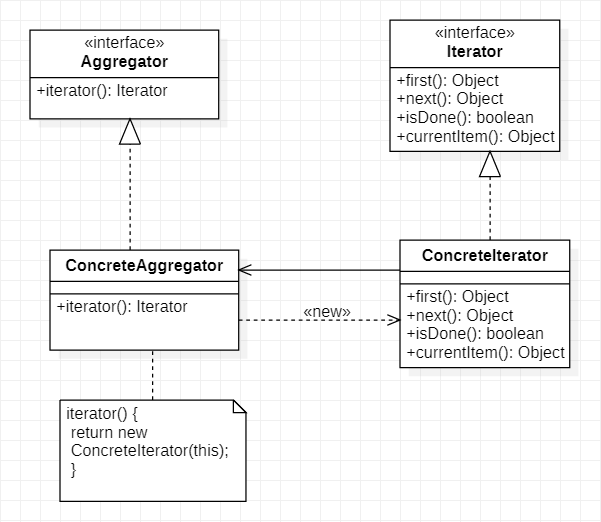
\includegraphics[scale=0.5]{IteratorClassDiagram.png}
\end{center}
\caption{Iterator Class Diagram}
\end{figure}

\begin{figure} [H]
\begin{center}
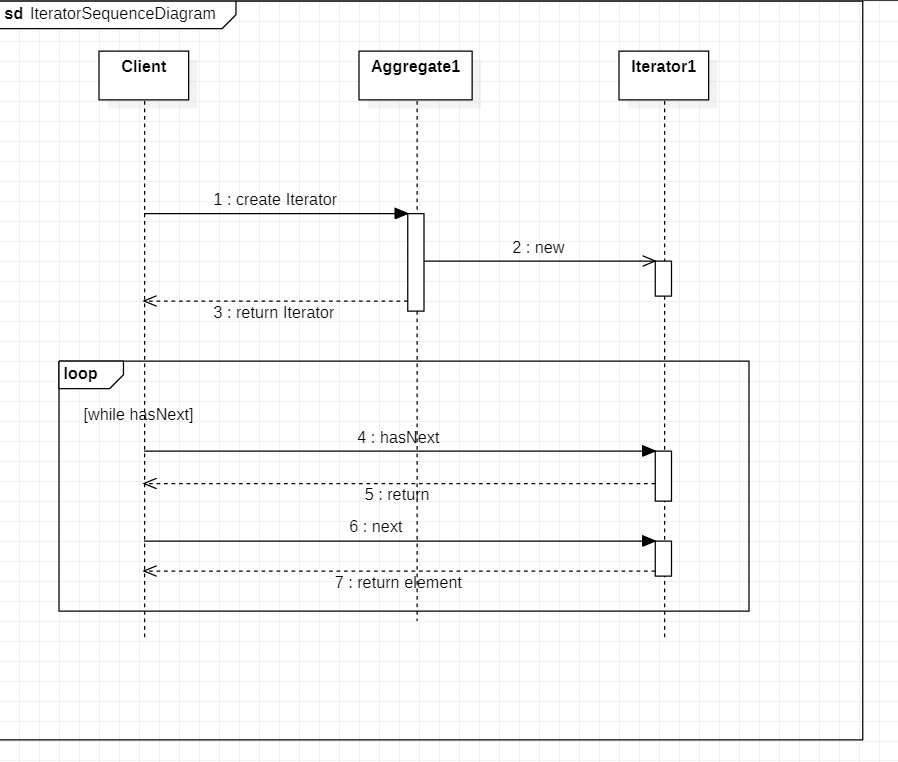
\includegraphics[scale=0.5]{IteratorSequenceDiagram.png}
\end{center}
\caption{Iterator Sequence Diagram}
\end{figure}

\subsubsection{Partecipanti}
Questo pattern è composto dai seguenti partecipanti:
\begin{itemize}
    \item Iterator: colui che espone i metodi di accesso alla struttura dati
    \item ConcreteIterator: implementa l’Iteratore e tiene il puntatore alla struttura dati
    \item Aggregator: definisce l’interfaccia per creare un oggetto di tipo Iteratore
    \item ConcreteAggregator: implementa l’interfaccia di creazione di un oggetto Iteratore
\end{itemize}
\subsubsection{Conseguenze}
Tale pattern presenta i seguenti vantaggi/svantaggi:
\begin{itemize}
  \item unica interfaccia di accesso: l’accesso ai dati avviene tramite l’Iterator che espone un’unica interfaccia e nasconde le diverse implementazioni degli Aggregator
  \item diversi iteratori di accesso: l’Aggregator può essere attraversato tramite diversi Iterator in cui ogni Iterator nasconde un algoritmo diverso
\end{itemize}

\subsection{Builder con Static Factory Method}
Il Builder design pattern è un pattern creazionale che permette di costruire oggetti complessi in modo facilitato, passo-passo. La responsabilità della creazione è delegata a una classe Builder, in genere una static inner class della classe di cui si vogliono costruire oggetti. Essa si bassa sulla fluent interface.
I metodi factory statici permettono di incapsulare la creazione di oggetti, tuttavia non sono un design pattern perché non astraggano dal tipo concreto di oggetto creato. Se presenti nella stessa classe che si vuole istanziare possono rappresentare un'alternativa ai costruttori, i quali diventano privati. Il vantaggio dei metodi factory statici è di rendere il codice più leggibile, in quanto possono avere nomi più significativi rispetto ai costruttori. Inoltre, essendo il costruttore privato, una sua futura modifica nella signature non va a "rompere" i client esistenti, basta modificare solo il codice della classe.  
\subsubsection{Struttura}
Ci sono diverse forme del Builde design pattern. Riporto un class Diagram più simile a quello utilizzato nel progetto.

\begin{figure} [H]
\begin{center}
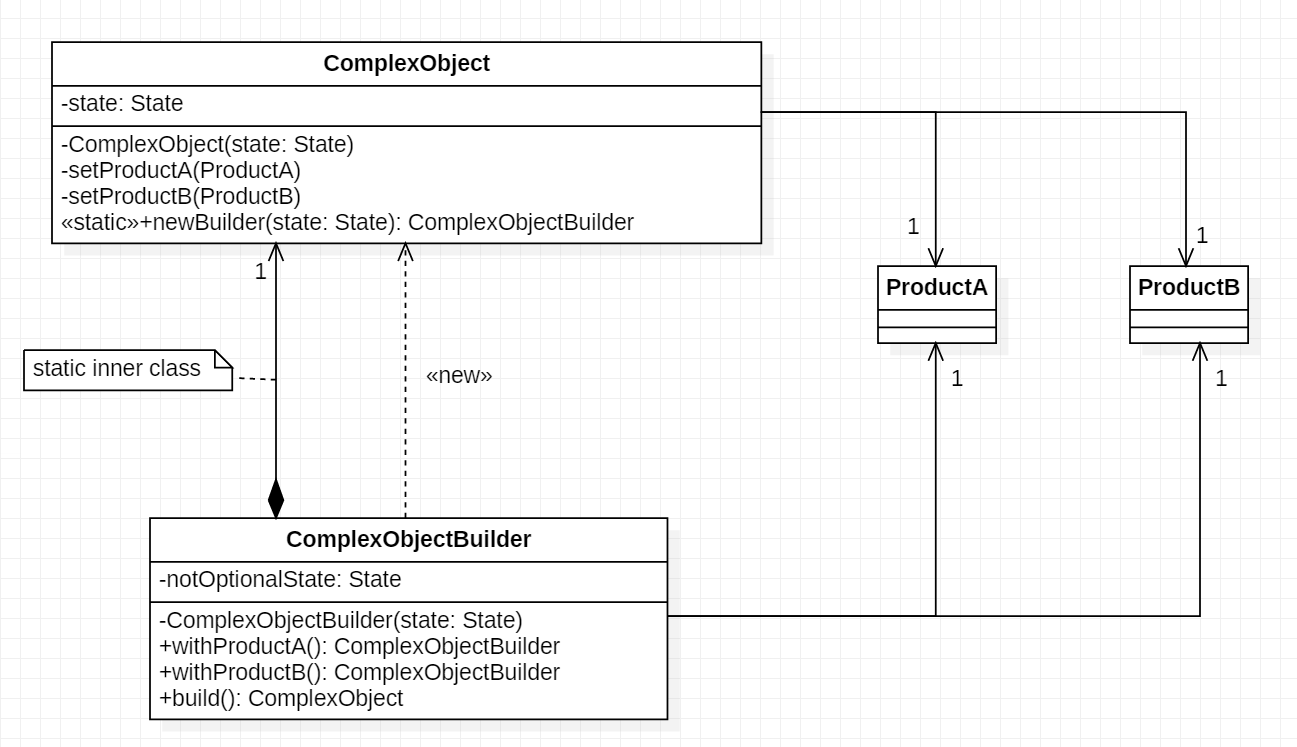
\includegraphics[scale=0.5]{BuilderClass.png}
\end{center}
\caption{Builder with static Factory Method Class Diagram}
\end{figure}

\subsubsection{Partecipanti}
\begin{itemize}
  \item ComplexObject: oggetto complesso che viene costruito dal ComplexObjectBuilder.
  \item ComplexObjectBuilder: costruisce e assembla le parti dell'oggetto complesso e tiene traccia della rappresentazione che crea.
\end{itemize}

\subsubsection{Conseguenze}
Tale pattern presenta i seguenti vantaggi/svantaggi:
\begin{itemize}
  \item La costruzione di un oggetto complesso e la sua rappresentazione vengono isolate.
  \item La creazione dell'oggetto complesso avviene in modo più semplice, leggibile e controllato.
  \item Lo svantaggio è che il codice risulta più complesso e più difficilmente modificabile.
\end{itemize}
\newpage 
\section{Progetto}

\section{Analisi dei Requisiti}
\subsection{Casi d'uso}
L'applicazione espone diverse funzioni che sono rese disponibili ad un Utente. Queste funzioni permettono di costruire nel programma un veicolo e attivargli la modalità di guida autonoma. La funzione di guida autonoma sottende l'inserimento della posizione corrente del veicolo e della posizione di destinazione.
L'Utente può inoltre gestire vari accessori elettrici del veicolo, quali il finestrino elettrico, il tergicristallo e lo specchietto retrovisore. 
\begin{figure} [H]
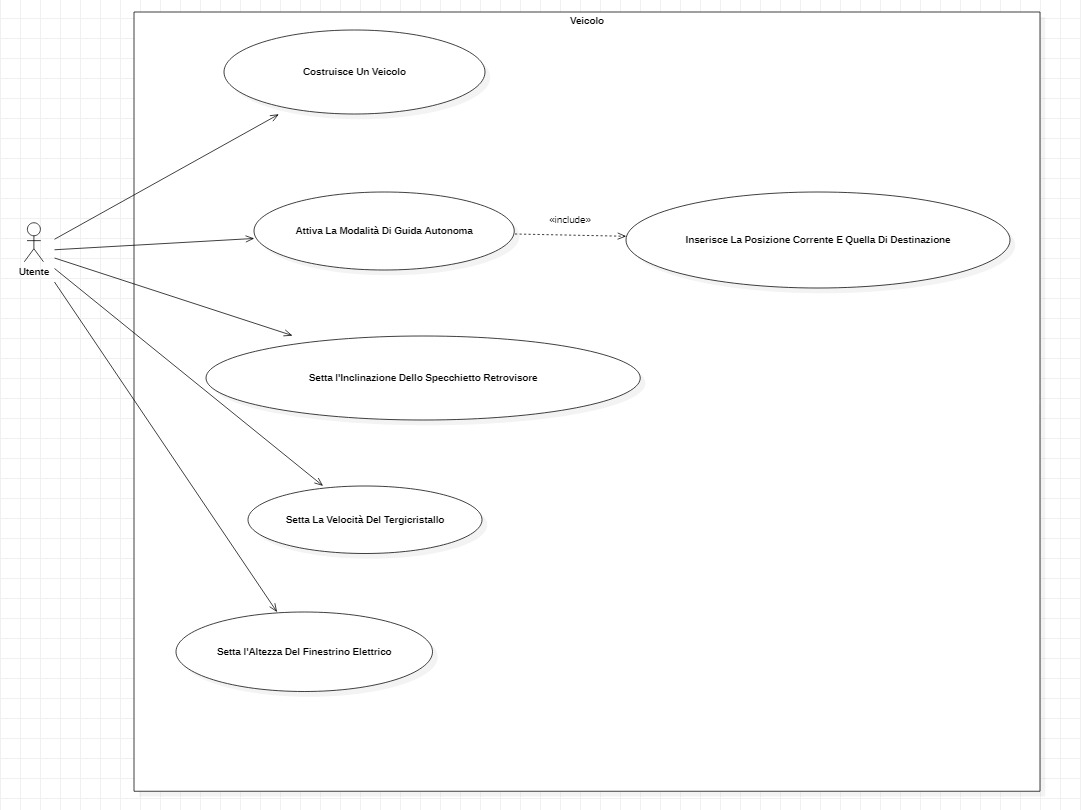
\includegraphics[width=1\textwidth,center]{UseCaseDiagram.png}
\caption{Use Case Diagram}
\end{figure}
\newpage 

\section{Progettazione}
Il progetto è strutturato dividendo il veicolo in sensori, attuatori e componenti che controllano gli attuatori rielaborando i dati forniti dai sensori. I sensori si occupano di estrarre informazioni dal mondo circostante. Questi dati vengono poi passati, per essere rielaborati, alle componenti intelligenti del sistema che impartiscono comandi agli attuatori. Gli attuatori compiono azioni sull'ambiente, grazie a quest'ultimi è possibile ad esempio manovrare il volante del veicolo per curvare o si possono fare azioni più ordinarie come abbassare il finestrino elettrico.
\subsection{Metodo}
Per la realizzazione è stato utilizzato il linguaggio di programmazione Java attraverso Eclipse. Sono state seguite vari fasi di sviluppo:
nella fase di analisi dei requisiti sono stati identificati i casi d'uso e rappresentati attraverso gli Use Case Diagrams. Nella struttura principale del programma sono stati usati i pattern Builder, Iterator e Observer. 


\subsection{Class Diagram}
Il Diagramma delle Classi in UML rappresenta la progettazione delle classi, esso mostra come vengono partizionate le responsabilità tra le classi.
Il Veicolo ha più Sensori e più Attuatori, fra cui gli attuatori per la guida autonoma (Attuatore del Freno, Acceleratore e Volante), e i Controllori per la gestione della guida autonoma e la gestione degli accessori.  
La Cpu tiene le collezioni dei Sensori e degli Attuatori del veicolo, oltre a un riferimento al Sistema di Navigazione. Essa genera Protocolli per il controllo della guida autonoma.
Il Protocollo è un insieme di Istruzioni sequenzializzate che gli Attuatori per la guida autonoma eseguono. 
L'ambiente circostante al veicolo è rappresentato come un Mappa 3D che contiene un insieme di Posizioni. Il Sistema di Navigazione contiene la Posizione corrente e quella di destinazione del veicolo.

\begin{figure} [H]
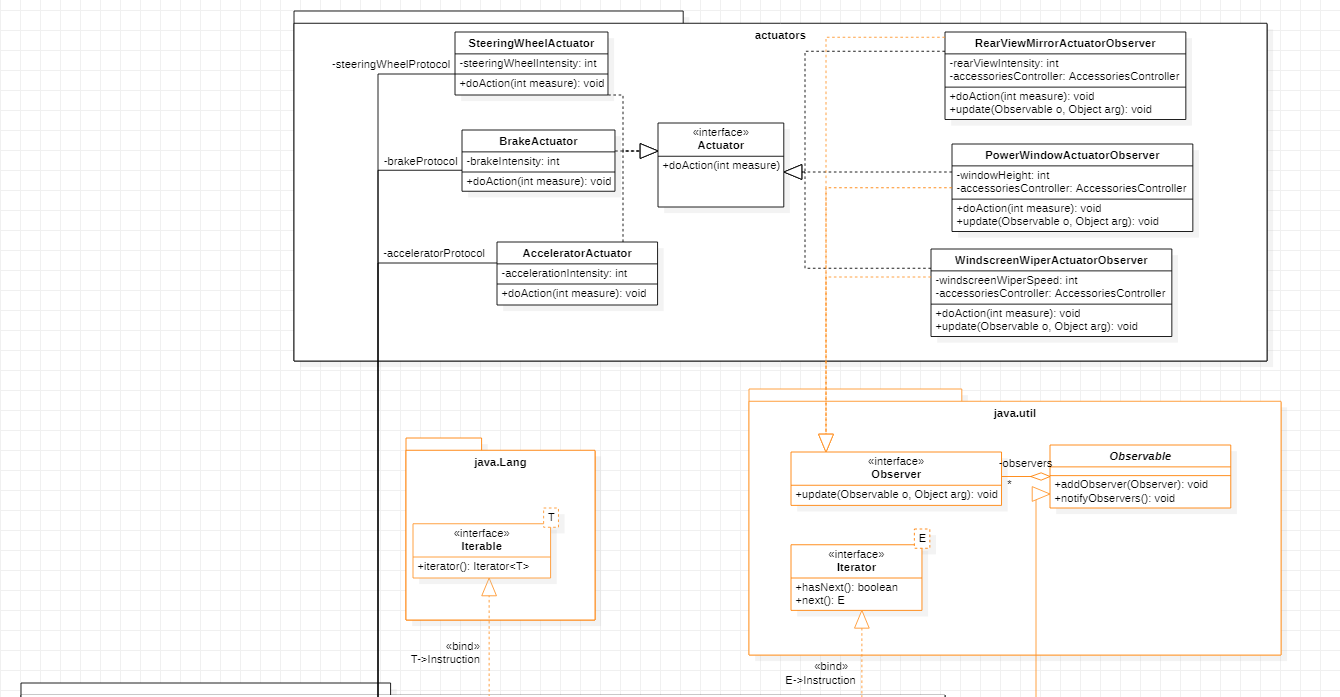
\includegraphics[width=1.3\textwidth,center]{part1.png}
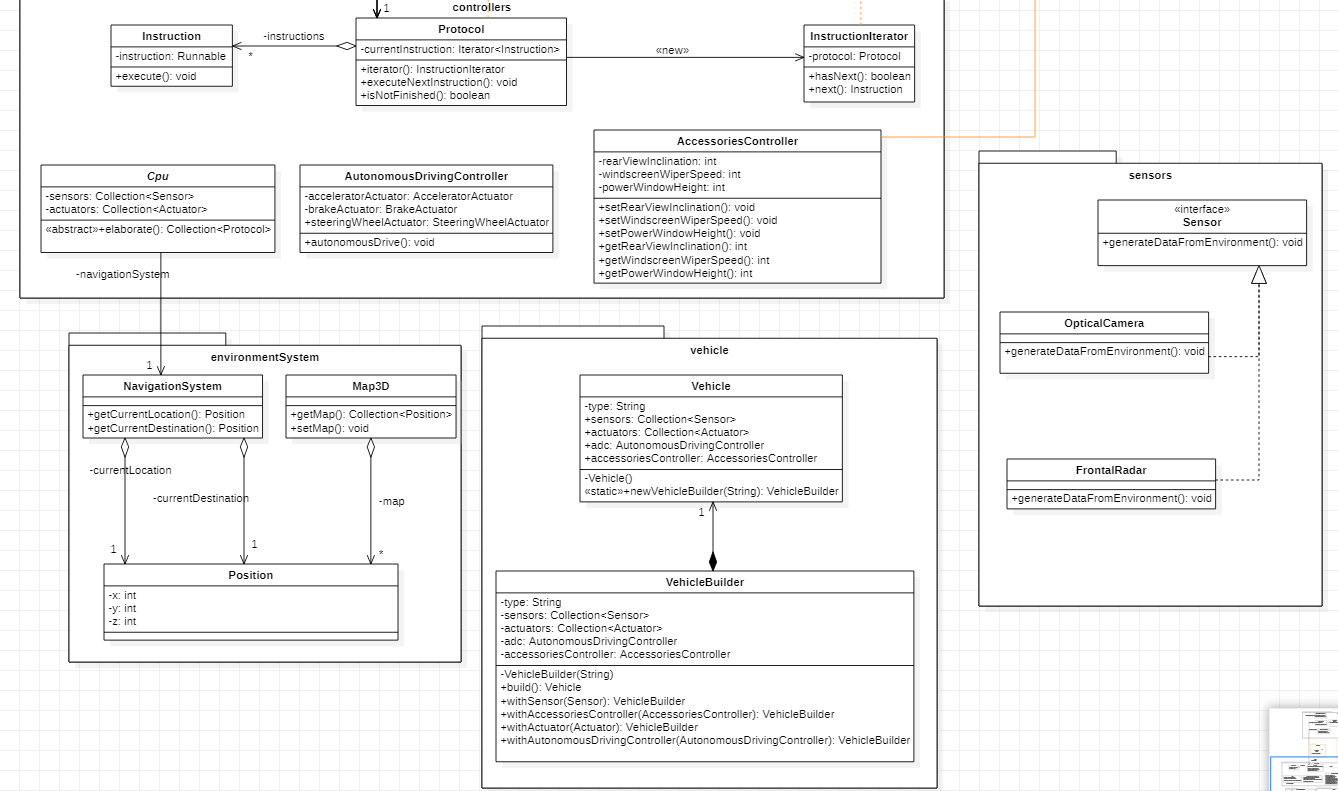
\includegraphics[width=1.3\textwidth,center]{part2.png}
\caption{Class Diagram}
\end{figure}

\newpage
\section{Implementazione}
Riporto l'organizzazione del codice in packages: 
\begin{figure} [H]
\begin{center}
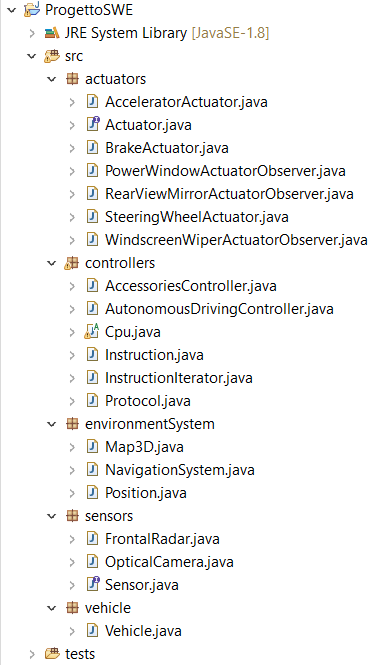
\includegraphics[scale=0.8]{Schema.png}
\end{center}
\caption{Organizzazione del codice in packages}
\end{figure}

Per l'implementazione sono state definite nuove classi ed interfacce o riutilizzate quelle della libreria standard (e.g. le interfacce  contenute nel package java.util come Iterator$\langle$E$\rangle$ e Observer).

\begin{itemize}
\item Instruction: ha un riferimento a una variabile di tipo Runnable (interfaccia funzionale) e il suo unico metodo execute() invoca il metodo run() della variabile d'istanza. 
\begin{figure} [H]
\begin{center}
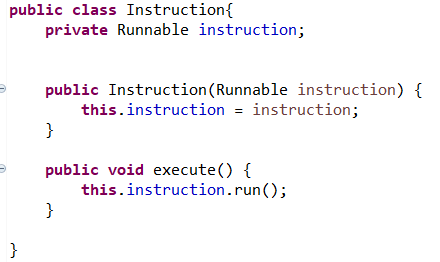
\includegraphics[scale=0.8]{Instruction.png}
\end{center}
\caption{Classe Instruction}
\end{figure}

\item InstructionIterator: implementa Iterator$\langle$Instruction$\rangle$, svolge il ruolo di ConcreteIterator nel design pattern Iterator. Implementa dunque i metodi next() e hasNext(). Contiene un riferimento a un Protocol, il ConcreteAggregator.
\begin{figure} [H]
\begin{center}
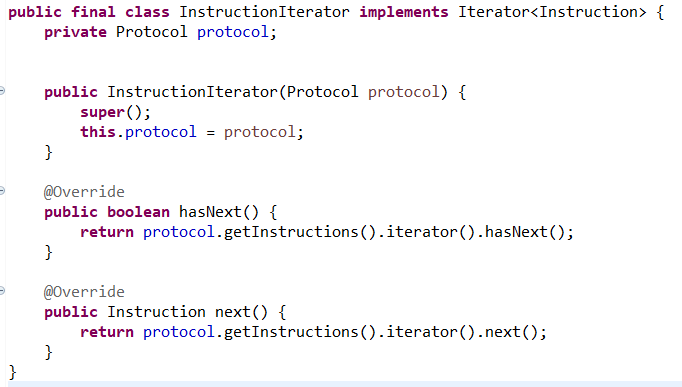
\includegraphics[scale=0.8]{InstructionIterator.png}
\end{center}
\caption{Classe InstructionIterator}
\end{figure}
\item Protocol: implementa Iterable$\langle$Instruction$\rangle$, svolge il ruolo di ConcreteAggregator nel design pattern Iterator. Implementa quindi il metodo iterator() che ritorna una nuova istanza della classe InstructionIterator(). Protocol contiene una collezione di Instruction e un riferimento all'Instruction corrente. Il metodo executeNextInstruction() esegue l'istruzione successiva a quella corrente. 
\begin{figure} [H]
\begin{center}
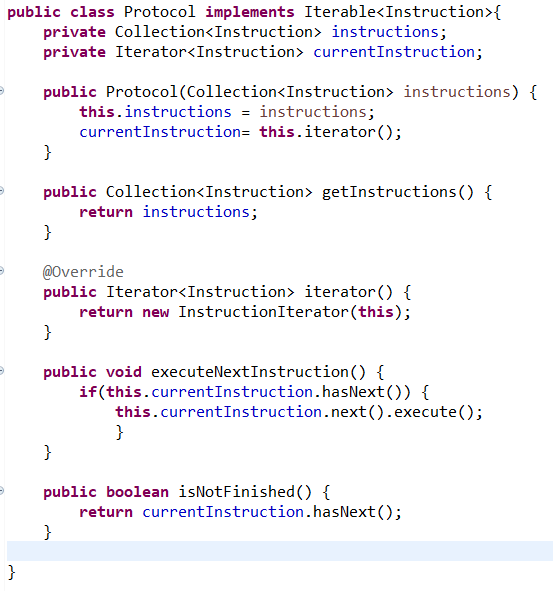
\includegraphics[scale=0.8]{Protocol.png}
\end{center}
\caption{Classe Protocol}
\end{figure}


\item AutonomousDrivingController: la sua responsabilità è di controllare, attraverso l'esecuzione di protocolli, gli attuatori del freno, volante e acceleratore per la guida autonoma del veicolo. Tiene infatti nello stato i riferimenti a questi attuatori. Il metodo autonomousDrive() esegue tutte le istruzioni dei protocolli precedentemente elaborati dalla classe Cpu. 

\begin{figure} [H]
\begin{center}
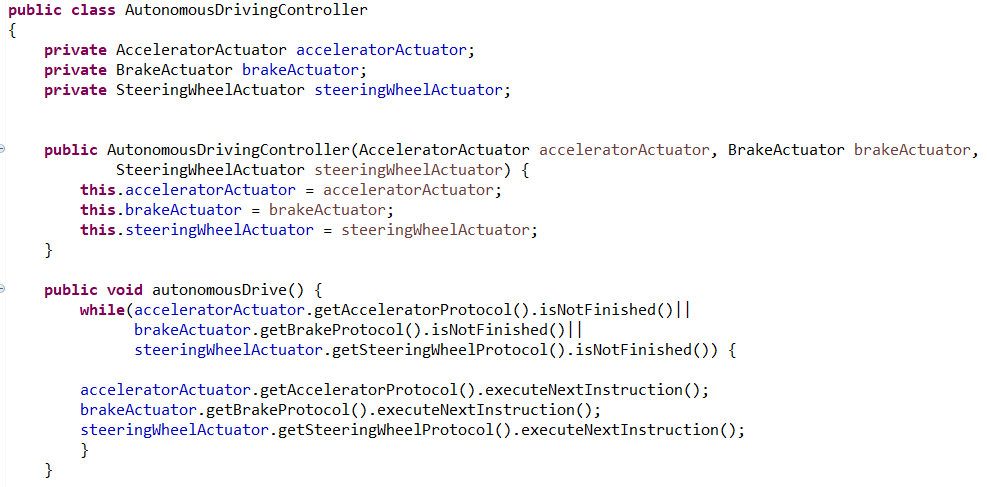
\includegraphics[scale=0.8]{AutonomousDrivingController.png}
\end{center}
\caption{Frammento di codice della classe AutonomousDrivingController}
\end{figure}
La classe astratta Cpu ha per stato i Sensori del veicolo, i suoi Attuatori e il Sistema di Navigazione. Il suo unico metodo astratto è elaborate() che restituisce un insieme di Protocolli.
\begin{figure} [H]
\begin{center}
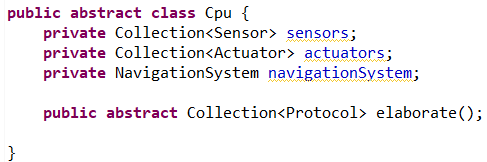
\includegraphics[scale=0.8]{Cpu.png}
\end{center}
\caption{Classe astratta Cpu}
\end{figure}

\item AccessoriesController: estende la classe Observable presente nel package java.util. Il suo stato contiene lo stato generale di tutti gli accessori della macchina, come l'altezza del finestrino elettrico e la velocità di movimento attuale del tergicristallo. Gli attuatori interessati (Observer) al cambiamento di stato di AccessoriesController sono PowerWindowActuatorObserver, RearViewMirrorActuatorObserver e WindscreenWiperActuatorObserver.
\begin{figure} [H]
\begin{center}
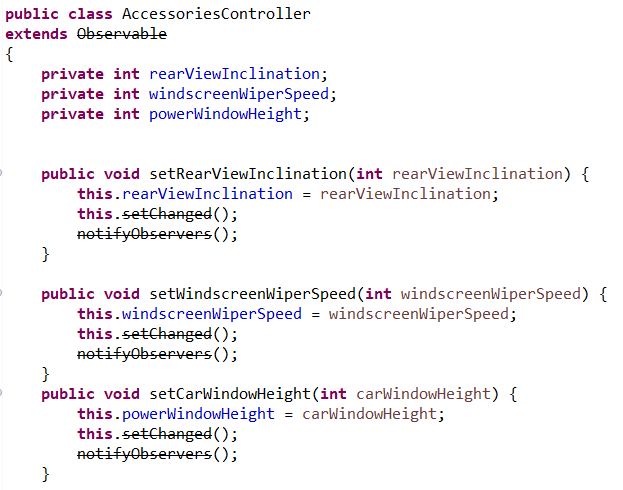
\includegraphics[scale=0.8]{AccessoriesController.png}
\end{center}
\caption{Frammento di codice della classe AccessoriesController}
\end{figure}


\item Sensor (interfaccia):  questa interfaccia rappresenta un generico sensore possibilmente presente nel veicolo ed ha un unico metodo generateDataFromEnvironment(). I Concrete Sensor implementano il metodo, in particolare:
    \begin{itemize}
    \item  OpticalCamera acquisisce dati come il colore del semaforo, 
    \item  FrontalRadar acquisisce dati per rilevare gli ostacoli presenti in strada
    \end{itemize}
\begin{figure} [H]
\begin{center}
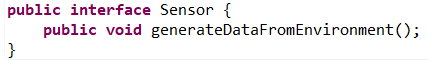
\includegraphics[scale=0.8]{Sensor.png}
\end{center}
\caption{Classe Sensor}
\end{figure}
    
    
\item Actuator (interfaccia): questa interfaccia rappresenta un generico attuatore possibilmente presente nel veicolo ed ha un unico metodo doAction(int measure). I Concrete Actuator implementano il metodo, in particolare:
    \begin{itemize}
    \item BrakeActuator agisce sull'intensità del freno , 
    \item AcceleratorActuator agisce sull'intensità dell'acceleratore, 
    \item SteeringWheelActuator agisce sull'inclinazione del volante, 
    \item PowerWindowActuatorObserver agisce sull'altezza del finestrino elettrico, 
    \item RearViewMirrorActuatorObserver agisce sull'inclinazione del finestrino retrovisore,  
    \item WindscreenWiperActuatorObserver agisce sulla velocità del tergicristallo. 
    \end{itemize}
Ad invocare il metodo possono essere le classi Controller del veicolo, ovvero AutonomousDrivingController e AccessoriesController.
\begin{figure} [H]
\begin{center}
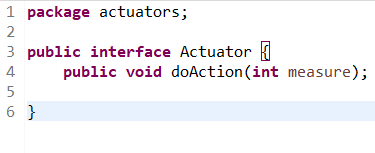
\includegraphics[scale=0.8]{Actuator.png}
\end{center}
\caption{Frammento di codice interfaccia Actuator}
\end{figure}

Dei ConcreteActuator, quelli necessari per la guida automa (BrakeActuator, AcceleratorActuator e SteeringWheelActuator) hanno inoltre un riferimento a una variabile di tipo Protocol. Ciascun protocollo verrà eseguito dal metodo autonomousDrive() della classe AutonomousDrivingController. 
\begin{figure} [H]
\begin{center}
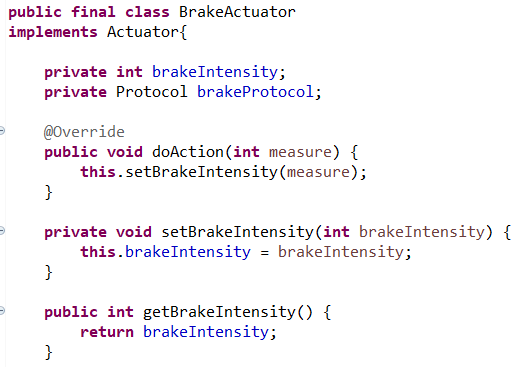
\includegraphics[scale=0.8]{BrakeActuator.png}
\end{center}
\caption{Frammento di codice della classe BrakeActuator}
\end{figure}

I ConcreteActuator inerenti invece agli accessori elettrici del veicolo  implementano inoltre l'interfaccia Observer, svolgendo il ruolo di ConcreteObserver nel design pattern Observer (con la classe AccessoriesController come Observable). Il metodo update() evoca doAction(int).
\begin{figure} [H]
\begin{center}
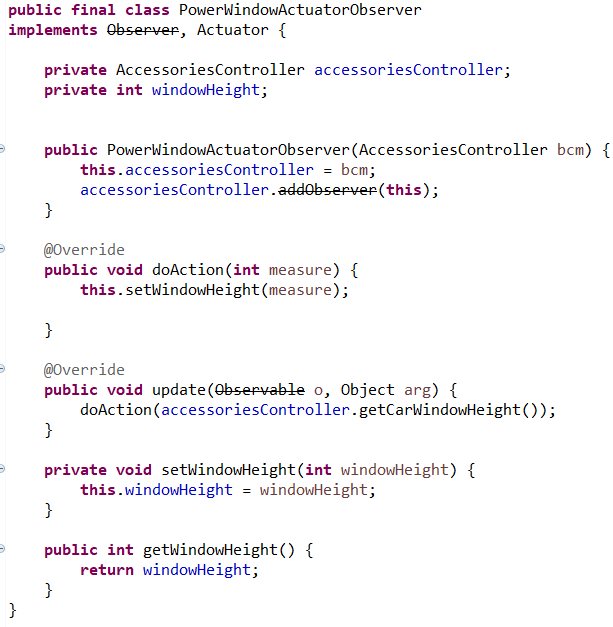
\includegraphics[scale=0.8]{PowerWindowActuatorObserver.png}
\end{center}
\caption{Classe PowerWindowActuatorObserver}
\end{figure}

\item Vehicle: è una classe complessa da istanziare utilizzando il design pattern Builder con la classe interna statica VehicleBuilder. Ha il costruttore e i metodi setter privati, ma accessibili a VehicleBuilder. Il costruttore prende come unico elemento una stringa per la tipologia di veicolo, gli altri attributi (collezione di Sensori, di Attuatori e un riferimento a un AutonomousDrivingController e a AccessoriesController) sono opzionali e assemblati attraverso i metodi with di VehicleBuilder. 
La classe statica interna VehicleBuilder ha lo stesso stato di Vehicle e un costruttore che prende sempre una stringa. I metodi with permettono di modificare lo stato interno di VehicleBuilder e alla fine, con il metodo build(), si andrà a creare una nuova istanza di Vehicle con lo stato analogo a quello di VehicleBuilder.

\begin{figure} [H]
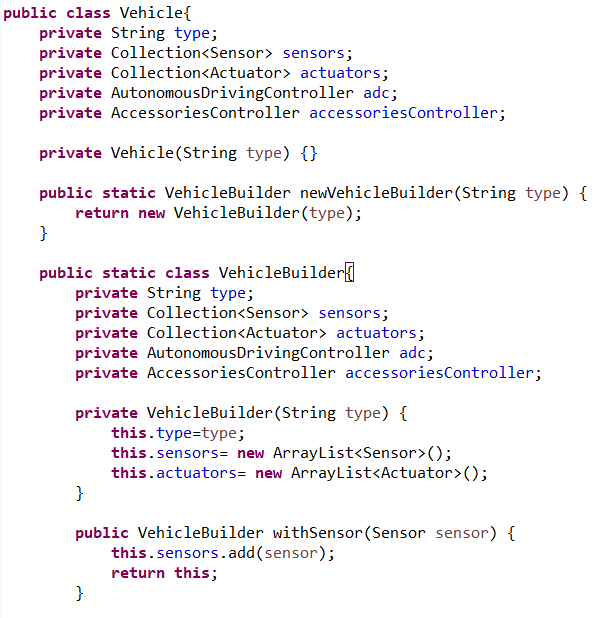
\includegraphics[scale=0.6]{Vehicle1.png}
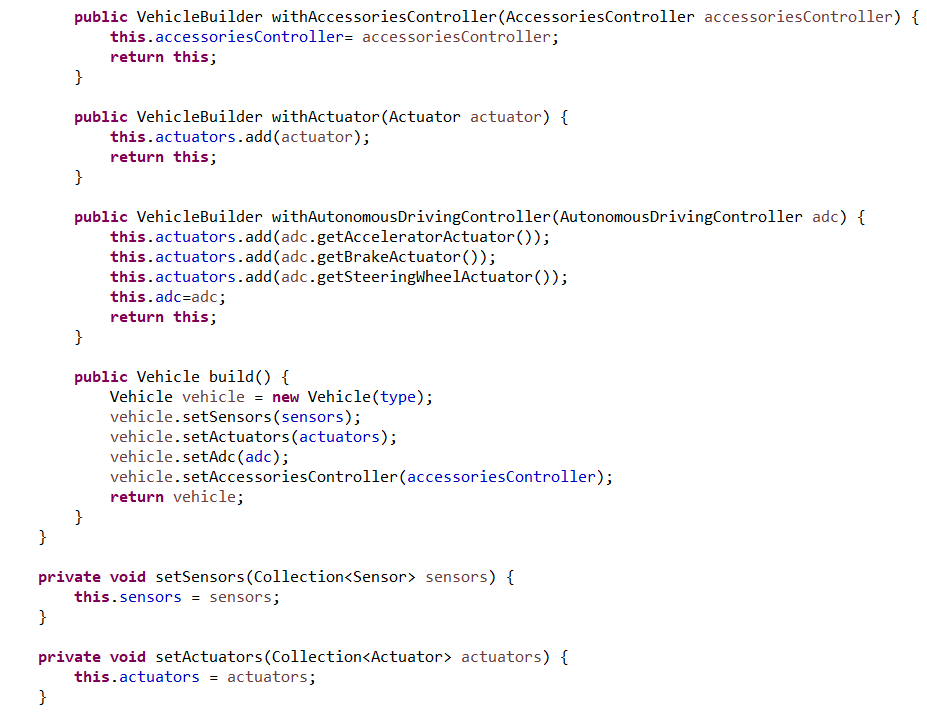
\includegraphics[scale=0.6]{Vehicle2.png}
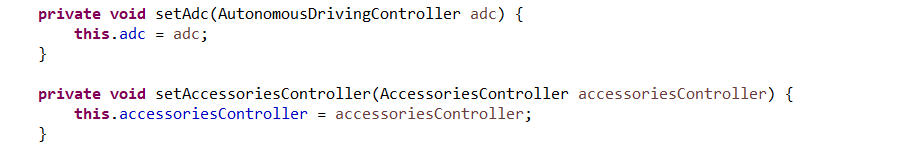
\includegraphics[scale=0.6]{Vehicle3.png}
\caption{Classi Vehicle e VehicleBuilder}
\end{figure}


\item Position: contiene per stato le coordinate di un qualsiasi oggetto che ha un riferimento a questa classe.
\begin{figure} [H]
\begin{center}
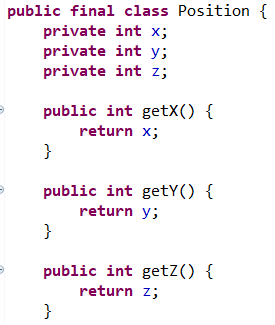
\includegraphics[scale=0.8]{Position.png}
\end{center}
\caption{Frammento di codice della classe final Position}
\end{figure}

La classe final Map3D contiene una collezione di Posizioni e fornisce i metodi getter e setter sulla collezione.
La classe NavigationSystem contiene nello stato due variabili di tipo Position che rappresentano la posizione corrente del veicolo e quella di destinazione.
\begin{figure} [H]
\begin{center}
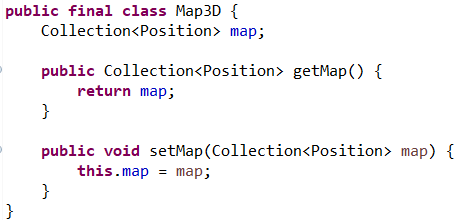
\includegraphics[scale=0.8]{Map3D.png}
\end{center}
\caption{Frammento di codice della classe final Map3D}
\end{figure}

\begin{figure} [H]
\begin{center}
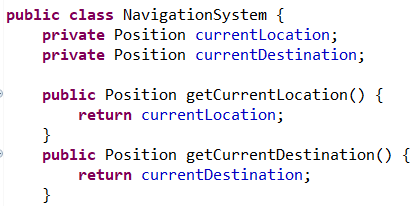
\includegraphics[scale=0.8]{NavigationSystem.png}
\end{center}
\caption{Frammento di codice della classe NavigationSystem}
\end{figure}

\end{itemize}


\subsection*{Dettagli di implementazione}
il progetto è stato realizzato utilizzando Eclipse. Per l'unit testing invece è stato usato il framework JUnit 4.0.

\section{Unit Testing}
Nel progetto sono stati verificati porzioni di codice, come metodi o classi, attraverso test cases. Nei metodi dei test vengono verificate delle asserzioni elementari utilizzando per esempio "assertEquals","assertTrue" e "assertFalse" di JUnit. I test sono stati scelti in prospettiva strutturale, in modalità white-box.
Le classi di Test realizzate sono:
\begin{enumerate}
\item VehicleTest: in questa classe di test si è testata la classe Vehicle e VehicleBuilder. In particolare si è verificato che la creazione di Vehicle attraverso il pattern Builder avvenisse correttamente. I metodi testati sono:
\begin{itemize}
    \item  newVehicleBuilder(String type), metodo statico di Vehicle
    \item withSensor(Sensor), withActuator(Actuator), withAccessoriesController(AccessoriesController), withAutonomousDrivingController(AutonomousDrivingController) di VehicleBuilder
    \item build() di VehicleBuilder
\end{itemize}

\begin{figure} [H]
\begin{center}
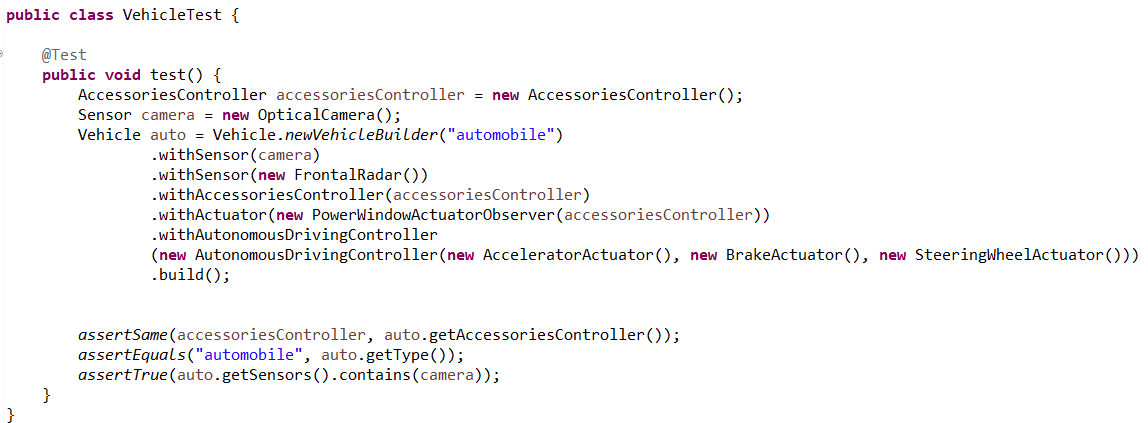
\includegraphics[scale=0.6]{VehicleTest.png}
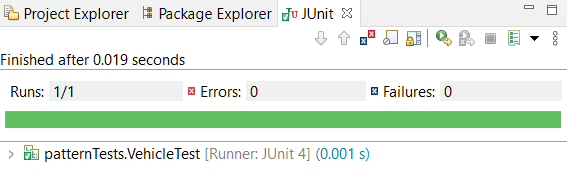
\includegraphics[scale=0.6]{VehicleTestJUnit.png}
\end{center}
\caption{VehicleTest}
\end{figure}

\item AccessoriesControllerTest: in questa classe di test si sono testati i metodi setter della classe AccessoriesController (Observable) e in particolare si è verificato il giusto comportamento del pattern Observer.
\begin{figure} [H]
\begin{center}
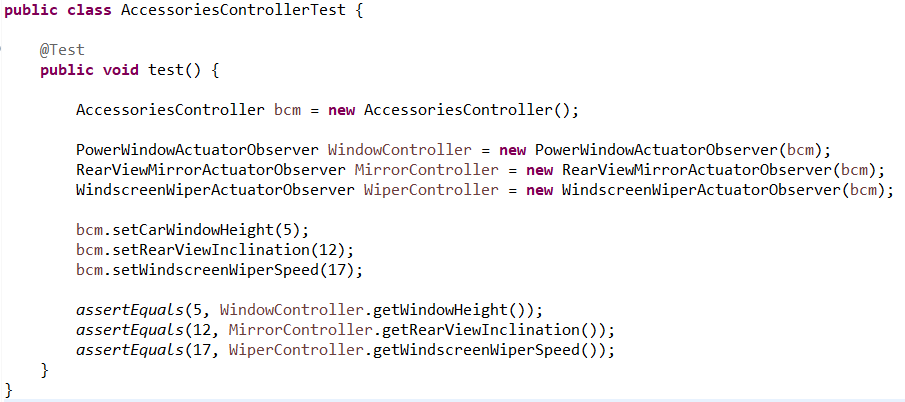
\includegraphics[scale=0.6]{AccessoriesControllerTest.png}
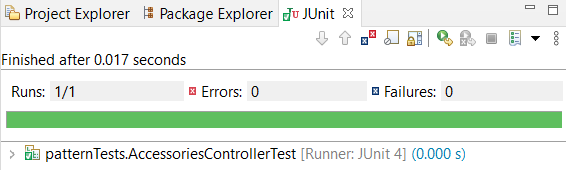
\includegraphics[scale=0.6]{AccessoriesControllerTestJUnit.png}
\end{center}
\caption{Accessories Controller Test}
\end{figure}

\item AutonomousDrivingControllerTest: in questa classe si test il metodo autonomousDrive() di AutonomousDrivingController. Vengono quindi creati i protocolli per il freno, acceleratore e volante e il metodo autonomousDrive() dovrà eseguirli.
\begin{figure} [H]
\begin{center}
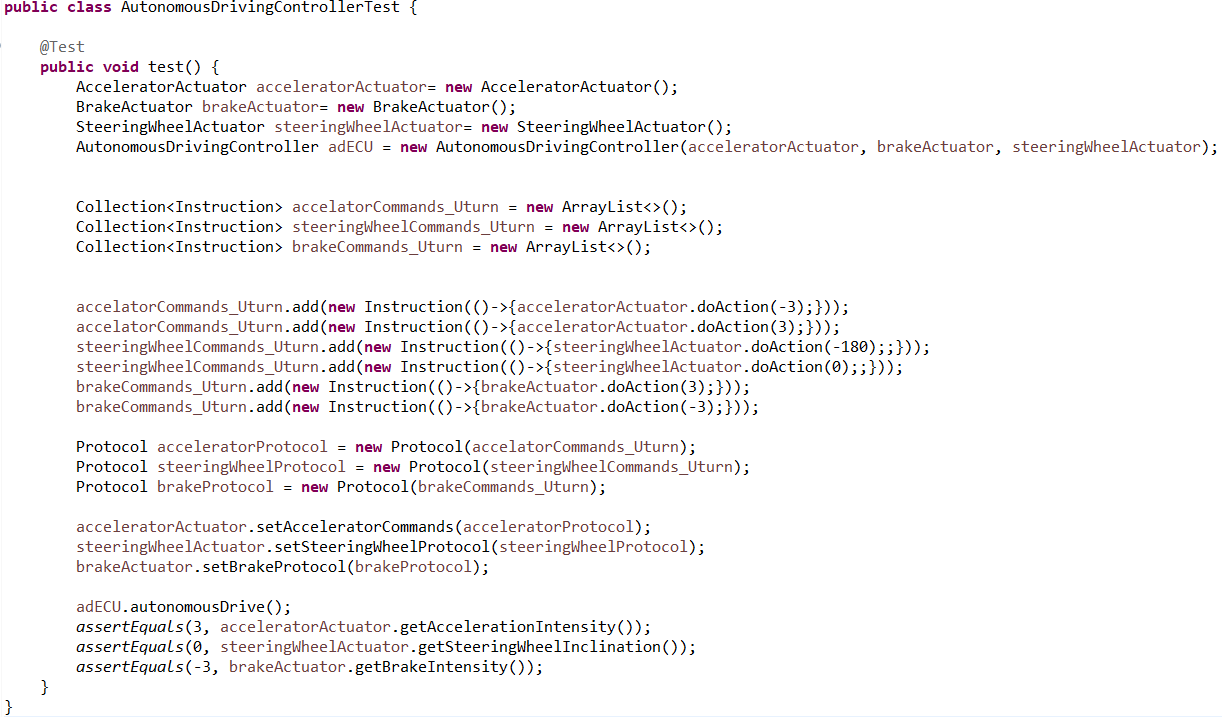
\includegraphics[scale=0.6]{AutonomousDrivingControllerTest.png}
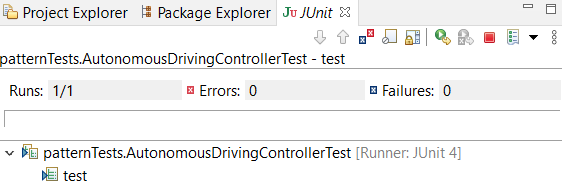
\includegraphics[scale=0.6]{AutonomousDrivingControllerTestJUnit.png}
\end{center}
\caption{VehicleTest}
\end{figure}
\end{enumerate}


\end{document}
